%\addcontentsline{toc}{chapter}{Introduction}
\section{Introduction}

This chapter presents the description of the system created for this Bachelor's Thesis. The solution proposed implements a software capable of tracking the user's hands and learning and recognizing the objects that are hand-held. 
\\
The system has two main parts: the software and the hardware. 
The hardware needed for the software to work correctly is an RGB-D sensor. In the following section the different data acquisition devices are explained and why it was decided to use an RGB-D sensor as the input of the system. 

 
\begin{figure}[h]
	\begin{center}
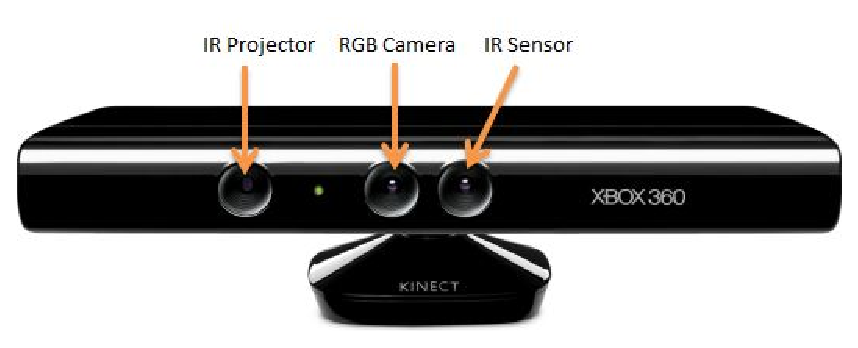
\includegraphics[scale=0.5]{img/kinect/kinect2.eps}
	\caption[Kinect Sensors]{Kinect sensors: depth sensor and VGA camera location.}
	\end{center}
\end{figure}
